\section{Auswertung}
\label{sec:Auswertung}

\subsection{Gedämpfte harmonische Schwingung}

Zunächst werden die Daten aus \autoref{tab:zeit-amplitude} geplottet, wobei die Ampltiude logarithmisiert werden.
Über diese wird ein Fit der Form

\begin{equation}
    ln(U_C) = ax + b
\end{equation}

gelegt. Der entstehende Graph ist in \autoref{fig:zeit-amplitude} zu sehen. 

\begin{table}[!htp]
\centering
\caption{Die Daten der Amplitudenmessung bei der gedämpften Schwingung.}
\label{tab:zeit-amplitude}
\begin{tabular}{S[table-format=3.0] S[table-format=1.2]}
\toprule
{$t$ / µs} & {$U$ / V} \\
\midrule
14 & 8.16 \\
27 & 6.80 \\
41 & 5.92 \\
54 & 4.96 \\
68 & 4.40 \\
81 & 3.60 \\
95 & 3.20 \\
108 & 2.72 \\
122 & 2.32 \\
136 & 2.00 \\
149 & 1.68 \\
162 & 1.44 \\
176 & 1.28 \\
189 & 1.12 \\
203 & 0.96 \\
217 & 0.80 \\
\bottomrule
\end{tabular}
\end{table}

\begin{figure}
    \centering
    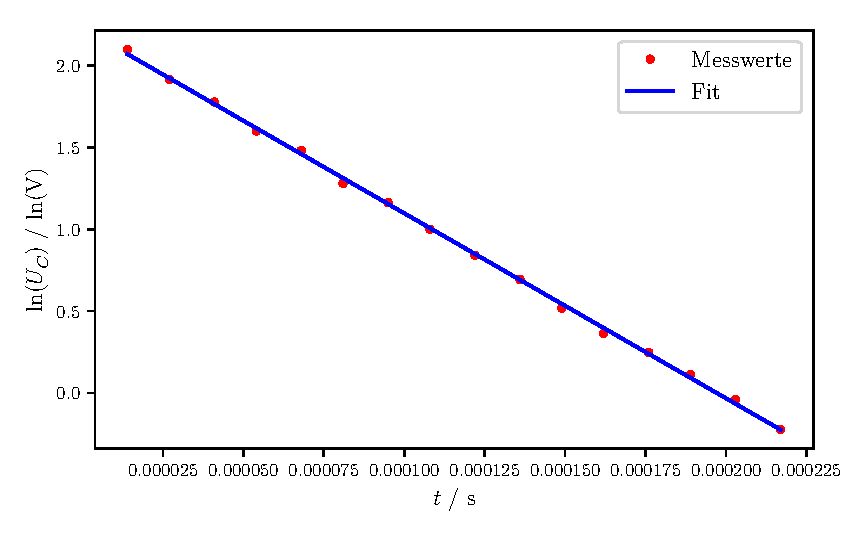
\includegraphics{build/plot-amplitude.pdf}
    \caption{Plot und Fit der logarithmisierten Ampltiude in Abhängikeit der Zeit.}
    \label{fig:zeit-amplitude}
\end{figure}

Die entsprechenden Parameter werden mittels Python 3.7.0 als

\begin{center}
    $a = (1,\~131 \pm 0,\~008) \cdot 10^{4} \frac{\ln(\symup{V})}{\symup{s}}$

    $b = (2,\~23 \pm 0,\~01) \ln(\symup{V})$
\end{center}

%TODO: Gleichung
bestimmt. Aus GLEICHUNG folgt direkt, dass 

\begin{center}
    $R = a \cdot 2L = (79.8 \pm 0.9)$ $\symup{\Omega}$
\end{center}

gilt. Der zugehörige Fehler nach Gauß berechnet sich dabei nach

\begin{equation}
    \Delta R = 2 \sqrt{ \bigg( L \cdot \Delta a \bigg)^2 + \bigg( a \cdot \Delta L \bigg)^2 }.
\end{equation}

Der Wert für die Induktivität der Spule $L$ wurde angegeben und ist mit weiteren angegebenen Gerätedaten in \autoref{tab:geraetedaten} zu finden.

\begin{table}[!htp]
\centering
\caption{Die angegebenen Gerätedaten.}
\label{tab:geraetedaten}
\begin{tabular}{S[table-format=1.2] @{${}\pm{}$} S[table-format=1.2] S[table-format=1.3] @{${}\pm{}$} S[table-format=1.3] S[table-format=2.1] @{${}\pm{}$} S[table-format=1.1] S[table-format=3.1] @{${}\pm{}$} S[table-format=1.1]}
\toprule
\multicolumn{2}{c}{$L$ / mH} & \multicolumn{2}{c}{$C$ / nF} & \multicolumn{2}{c}{$R_1$ / $\symup{\Omega}$} & \multicolumn{2}{c}{$R_2$ / $\symup{\Omega}$} \\
\midrule
3.53 & 0.03 & 5.015 & 0.015 & 30.3 & 0.1 & 271.6 & 0.3 \\
\bottomrule
\end{tabular}
\end{table}

%%%%%%%%%%%%%%%%%%%%%%%%%%%%%%%%%%%%%%%%%%%%%%%%%%%%%%
\subsection{Aperiodischer Grenzfall}

%TODO: Gleichung
Nach GLEICHUNG ergibt sich der errechnete Wert für den Widerstand, mit dem der aperiodische Grenzfall erreicht wird, als

\begin{center}
    $R_\text{Theorie} = (1678 \pm 8)$ $\symup{\Omega}$,
\end{center}

wobei sich der Fehler nach Gauß aus %R = 2*sqrt(L/C)

\begin{equation}
    \Delta R_\text{ap} = \sqrt{ \frac{C}{L} \cdot \bigg( \frac{L}{C^2} \cdot \Delta C \bigg)^2 + \frac{C}{L} \cdot \bigg( \frac{1}{C} \cdot \Delta L \bigg)^2 }
\end{equation}

berechnet.

Der durch Variation des Widerstandes Wert wird als

\begin{center}
    $R_\text{ap} = (1355 \pm 5)$ $\symup{\Omega}$
\end{center}

bestimmt.

%%%%%%%%%%%%%%%%%%%%%%%%%%%%%%%%%%%%%%%%%%%%%%%%%%%%%%
\subsection{Bestimmung der Güte mittels variabler Frequenz}

%TODO: Gleichung
Die gemessenen Werte sind in \autoref{tab:var-freq} zu finden. Diese werden zur Veranschaulichung in einem Plot aufgetragen, dabei werden die Frequenzen $f$ nach $\omega = 2 \pi f$ in Kreisfrequenzen umgerechnet.
Die Theoriekurve, die sich nach GLEICHUNG berechnet, wird in diesem Plot ebenfalls aufgetragen.

\begin{table}[!htp]
\centering
\caption{Die Amplituden und Phasenverschiebung in Frequenzabhänigkeit mit $U_0 = 6.55$ V.}
\label{tab:var-freq}
\begin{tabular}{S[table-format=2] S[table-format=2.1] S[table-format=1.2]}
\toprule
{$f$ / kHz} & {$U_C$ / V} & {$\Delta t$ / µs} \\
\midrule
12 & 7.2 & 1.2 \\
14 & 7.8 & 1.5 \\
16 & 8.1 & 1.5 \\
18 & 8.3 & 1.6 \\
20 & 9.0 & 1.7 \\
22 & 9.5 & 1.8 \\
24 & 10.3 & 2.2 \\
26 & 11.3 & 2.5 \\
28 & 12.4 & 2.9 \\
30 & 13.8 & 3.4 \\
32 & 15.2 & 4.2 \\
33 & 16.0 & 4.6 \\
34 & 16.5 & 5.1 \\
35 & 16.8 & 5.6 \\
36 & 16.8 & 6.3 \\
37 & 16.5 & 6.8 \\
38 & 15.9 & 7.3 \\
39 & 15.1 & 7.7 \\
40 & 14.2 & 8.0 \\
41 & 13.2 & 8.2 \\
42 & 12.2 & 8.3 \\
44 & 10.5 & 8.5 \\
46 & 9.0 & 8.5 \\
48 & 7.5 & 8.4 \\
50 & 6.5 & 8.28 \\
52 & 5.7 & 8.08 \\
54 & 5.1 & 7.84 \\
56 & 4.6 & 7.72 \\
58 & 4.1 & 7.48 \\
60 & 3.7 & 7.28 \\
62 & 3.4 & 7.08 \\
\bottomrule
\end{tabular}
\end{table}

\begin{figure}
    \centering
    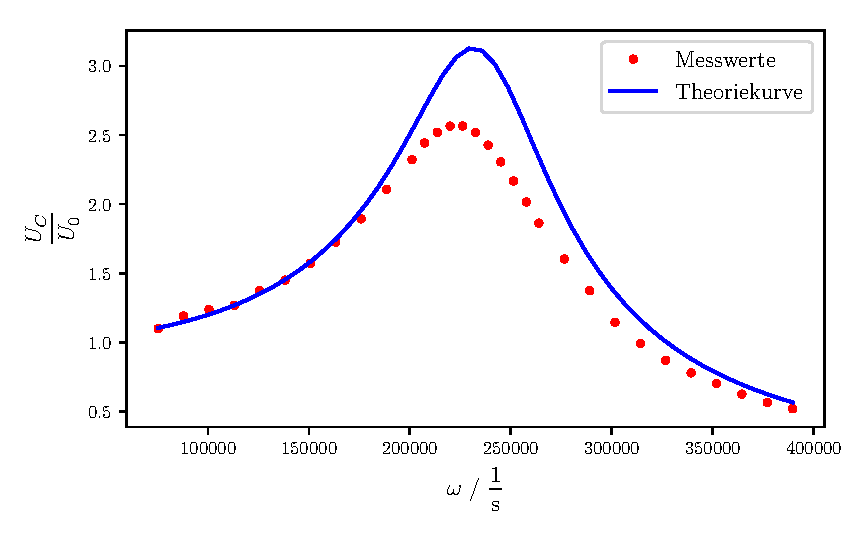
\includegraphics{build/plot-guete.pdf}
    \caption{Plot und Theoriekurve des Amplitudenverhältnis gegen die Frequenz aufgetragen.}
    \label{fig:guete}
\end{figure}

Aus diesen Daten lässt sich die Güte $q_\text{exp}$ durch Ablesen als

\begin{center}
    $q_\text{exp} = 2,\~56$
\end{center}

%TODO: Gleichung
bestimmen. Der zugehörige Theoriewert berechnet sich nach GLEICHUNG als

\begin{center}
    $q_\text{theo} = 3,\~09 \pm 0,\~01$.
\end{center}

Der Fehler nach Gauß berechnet sich dabei nach

\begin{equation}
    \Delta q_\text{theo} = \sqrt{\cdot \frac{L}{C}} \cdot \sqrt{ \bigg( \frac{1}{R^2} \cdot \Delta R \bigg)^2 + \bigg(\frac{1}{2RC} \cdot \Delta L \bigg)^2 + \bigg(\frac{L}{2RC^2} \cdot \Delta C \bigg)^2}.
\end{equation}

Die Resonanzfrequenz wird nach GLEICHUNG als

\begin{center}
    $\omega_\text{res} = (2,\~314 \pm 0,\~001) \cdot 10^{5}$ $\frac{1}{s}$
\end{center}

bestimmt, wobei sich der zugehörige Fehler nach Gauß nach

\begin{equation}
    \Delta \omega_\text{res} = \dfrac{1}{\sqrt{\frac{1}{LC} - \frac{R^2}{2L^2}}} \cdot \sqrt{ \bigg( \frac{R}{2L^2} \cdot \Delta R \bigg)^2 + \bigg( \frac{L - CR^2}{2CL^3} \cdot \Delta L \bigg)^2 + \bigg( \frac{1}{2LC^2} \cdot \Delta C \bigg)^2 }
\end{equation}

berechnet. Der zur experimentellen Bestimmung der Resonanzfrequenz wird die Stelle der maximalen Ampltiude abgelesen.
Diese beträgt

\begin{center}
    $\omega_\text{res} = 2,\~2 \cdot 10^{5}$ $\frac{1}{\symup{s}}$.
\end{center}


%TODO: Gleichung
Die Frequenzen $\omega_1$ und $\omega_2$ bei denen die Phasenverschiebung $\frac{\pi}{4}$ beziehungsweise $\frac{3\pi}{4}$ beträgt, 
berechnen sich nach GLEICHUNG als

\begin{center}
    $\omega_1 = (2,\~79 \pm 0,\~01) \cdot 10^{5}$ $\frac{1}{\symup{s}}$

    $\omega_2 = (2,\~022 \pm 0,\~008) \cdot 10^{5}$ $\frac{1}{\symup{s}}$.
\end{center}

Der Fehler nach Gauß errechnet sich dabei nach

\begin{equation}
    \Delta \omega_{1,2} = \sqrt{\bigg( \frac{\partial \omega_{+,-}}{\partial C} \cdot \Delta C \bigg)^2 + \bigg( \frac{\partial \omega_{+,-}}{\partial L} \cdot \Delta L \bigg)^2 + \bigg( \frac{\partial \omega_{+,-}}{\partial R} \cdot \Delta R \bigg)^2}, 
\end{equation}

wobei die einzelnen partiellen Ableitungen im Folgenden aufgeführt sind:

\begin{center}
    $\bigg( \frac{\partial \omega_{1,2}}{\partial C} \bigg)^2 = \Bigg( \dfrac{1}{2L\sqrt{\frac{1}{LC}+\frac{R^2}{4L^2}}C^2} \Bigg)^2$

    $\bigg( \frac{\partial \omega_{1,2}}{\partial R} \bigg)^2 = \Bigg( \dfrac{R}{4L^2\sqrt{\frac{R^2}{4L^2}+\frac{1}{CL}}} \pm \dfrac{1}{2L} \Bigg)^2$

    $\bigg( \frac{\partial \omega_{1,2}}{\partial L} \bigg)^2 = \Bigg( \mp \dfrac{R}{2L^2}+\dfrac{-\frac{1}{CL^2}-\frac{R^2}{2L^3}}{2\sqrt{\frac{1}{CL}+\frac{R^2}{4L^2}}} \Bigg)^2$.
\end{center}

\begin{figure}
    \centering
    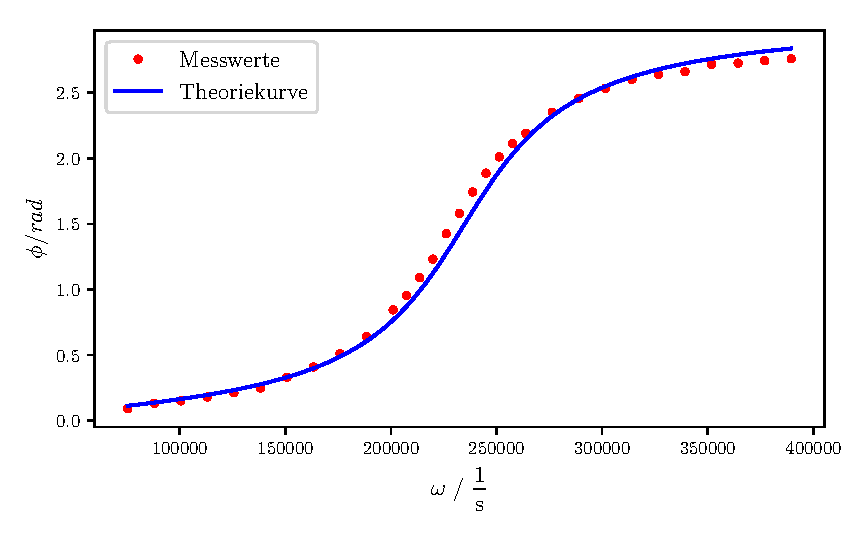
\includegraphics{build/plot-phase.pdf}
    \caption{Plot und Theoriekurve des Phasenunterschiedes gegen die Frequenz aufgetragen.}
    \label{fig:phase}
\end{figure}

%TODO: Gleichung
Um die experimente$\omega_1 = 2,\~1 \cdot 10^{5}$ $\frac{1}{\symup{s}}$

    $\omega_2 = 2,\~8 \cdot 10^{5}$ $\frac{1}{\symup{s}}$.llen Werte zu bestimmen, werden die Werte in \autoref{tab:var-freq} in einem Plot aufgetragen. Des Weiteren wird in diesem die Theoriekurve, die sich nach GLEICHUNG berechnet, aufgetragen.
Der entsprechende Plot ist in \autoref{fig:phase} zu sehen.
Daraus werden die Werte für die Frequenzen abgelesen, bei denen die Phasenverschiebung $\frac{\pi}{4}$ beziehungsweise $\frac{3\pi}{4}$ beträgt. 
Diese lauten

\begin{center}
    $\omega_1 = 2,\~1 \cdot 10^{5}$ $\frac{1}{\symup{s}}$

    $\omega_2 = 2,\~8 \cdot 10^{5}$ $\frac{1}{\symup{s}}$.
\end{center}
